\begin{multicols*}{2}
\section{\tcblst{tcolorbox} 代码块测试}

\subsection{\tcblst{tcolorbox} 代码块测试}

\subsubsection{\tcblst{tcolorbox} 代码块测试}

\begin{tcblisting}{
  mycode/betweenline={test.tex},
  mycode/betweenline/syntax={latex},
  mycode/betweenline/highlightlines={5-7},
  listing only,
  listing above text
}
% comments
% comments
% comments
% comments
% comments
% comments


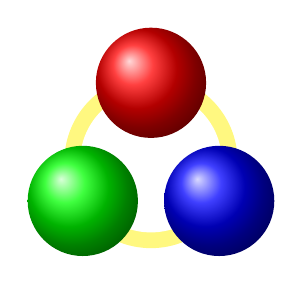
\begin{tikzpicture}
\path[fill=yellow!50!white] (0,0) circle (11mm);
\path[fill=white] (0,0) circle (9mm);
\foreach \w/\c in {90/red,210/green,330/blue}
{\path[shading=ball,ball color=\c] (\w:1cm) circle (7mm);}
\end{tikzpicture}
\end{tcblisting}

\begin{itemize}

\item 下面是一个列表测试项

\begin{tcblisting}{
  mycode/betweenline={test.hs},
  mycode/betweenline/syntax={haskell},
  mycode/betweenline/highlightlines={1-4},
  listing only,
}
module Main where

import Lib
import 脎\codeHL{Control}吡Control.Lens 

main :: IO ()
main = someFunc 

lst = [x| x <- ['a'..'z']] 
\end{tcblisting}

\end{itemize}

左侧的 \LaTeX 语言高亮似乎有些问题,这个应该是 Pygments 的锅\rlap。

\begin{tcblisting}{
  mycode/betweenline={test.rkt},
  mycode/betweenline/syntax={racket},
  mycode/betweenline/highlightlines={1-6},
  listing only,
}
;; 过程合约 :  in-S? : Natural   → Bool
;; 过程用途 : (in-S?     n   )   = #t 仅当 n 属于 S , 否则为 #f
;; 实参语法 :          Natural ::=  0 | (succ Natural)
(define in-S? 
  (lambda (n)
    (if (zero? n) #t
        (if (>= (- n 3) 0) (in-S? (- n 3))
            #f))))
\end{tcblisting}

泥濠!我是沉积岩!下面是一段一段测试文字:%
\tcblst[haskell]{lst = [x| x <- }
\tcblst[haskell]{['a'..'g']] -- by 沉积岩}\ 
\tcblst{tcolorbox}

\begin{tcblisting}{
  mycode/betweenline={test.lean},
  mycode/betweenline/syntax={lean4},
  mycode/betweenline/highlightlines={1-4},
  listing only,
}
theorem funext {f₁ f₂ : ∀ (x : α), β x} (h : ∀ x, f₁ x = f₂ x) : f₁ = f₂ := by
  show extfunApp (Quotient.mk' f₁) = extfunApp (Quotient.mk' f₂)
  apply congrArg
  apply Quotient.sound
  exact h
\end{tcblisting}

\end{multicols*}

\newpage